\documentclass{article}
\usepackage[utf8]{inputenc}
\usepackage{graphicx}
\graphicspath{ {./images/} }
\usepackage{multicol}
\usepackage[spanish, english]{babel}
\usepackage[left=3cm,right=3cm,top=3cm,bottom=3cm]{geometry}

\providecommand{\keywords}[1]{
  \small	
  \textbf{\textit{\quad \quad Keywords: }} #1}

\providecommand{\pclave}[1]{
  \small	
  \textbf{\textit{\quad \quad Palabras Clave: }} #1}
\usepackage{fancyhdr} 
\pagestyle{fancy} 
\fancyhead{} 
\fancyfoot{} 
\fancyhead[C]{DATA STORYTELLING EXAMPLES $\bullet$ Marzo 2022 $\bullet$ } 
\fancyfoot[RO,LE]{\thepage}

%Idiomas: \selectlanguage{english} \selectlanguage{spanish}

\begin{document}

\title{Trabajo Encargado N°1: DATA STORYTELLING EXAMPLES}
\begin{titlepage}
\begin{figure}[htb]
\begin{center}

\includegraphics[width=5cm]{logo.png}
\end{center}
\end{figure}
\vspace*{-0.25in}
\begin{center}
\large{UNIVERSIDAD PRIVADA DE TACNA}\\
\vspace*{-0.025in}
INGENIERIA DE SISTEMAS  \\

\vspace*{0.5in}
\begin{large}
TITULO:\\
\end{large}

\vspace*{0.1in}
\begin{Large}
\textbf{DATA STORYTELLING EXAMPLES} \\
\end{Large}

\vspace*{0.3in}
\begin{Large}
\textbf{CURSO:} \\
\end{Large}

\vspace*{0.1in}
\begin{large}
INTELIGENCIA DE NEGOCIOS\\
\end{large}

\vspace*{0.3in}
\begin{Large}
\textbf{DOCENTE:} \\
\end{Large}

\vspace*{0.1in}
\begin{large}
 Ing. Patrick Cuadros Quiroga\\
\end{large}

\vspace*{0.2in}
\vspace*{0.1in}
\begin{large}

Integrantes: \\
\begin{flushleft}
Briset Celia Garcia Salazar\hfill(2018062496) \\
Diego Manuel Gorbeño Mamani\hfill(2018000354)\\
Luis Fernando Flores Querie\hfill(2018062394)\\

\end{flushleft}
\end{large}

\vspace*{0.1in}
\begin{large}
Tacna - Perú\\
2022
\end{large}
\end{center}
\end{titlepage}

\vspace*{\fill}
	
\begin{center}
    
\selectlanguage{english}
\begin{abstract}
Narrative in Data Visualization is one of the main Big Data tools that businesses cannot miss. For this reason, this article contains the most interesting aspects of Data Storytelling, what it is and how to improve results thanks to it.

In case you did not know, more and more big data professionals and storytellers are going to be needed in the sector. The change in the digital age demands profiles with analytical and business intelligence capabilities. As a consequence, the new generations will go beyond these disciplines, with new ideas and spaces for business.
\quad 

 \end{abstract}
 
 
 \keywords{}
 
Big Data, Data Storytelling
\end{center}
\vspace*{\fill}

\newpage 


\begin{multicols}{2}

\section{Introduction}
Over the past few years, data storytelling has taken off. This isn't only because data and the role it plays in our lives is increasing. It’s also because storytelling is the way we as humans have always come to understand ourselves and the world we live in.

Data storytelling is the concept of building a compelling narrative based on complex data and analytics which help support the message of your story to influence and inform a particular audience. It's very similar to human storytelling, but provides the added benefits of deeper insights and supporting evidence through graphs and charts.
 
\section{State of Art}

\subsection{Data Storytelling}
It's a technique that uses data to tell a story. It's a useful way of presenting information, which means it can be used with both internal and external audiences.
Data storytelling goes beyond representing data in a more engaging way. It's about showing how or why the data changed over a period of time, and to do that you need to put together:

\begin{itemize}
\item \textbf{ a narrative}
\item \textbf{ a context}
\item \textbf{characters}
\end{itemize}

\subsection{¿Why tell a story with data?}
 Big Data is already a reality and every day more and more companies are investing in a culture based on tangible and real evidence.
 With so much information available, data-driven storytelling is a way to organize it all and present it in a more enjoyable and accessible way.
Since it's easier to absorb information that way, data storytelling also makes your content have more shelf life and generate more engagement, whether it's shared online or generates word-of-mouth marketing.
Several studies show that datastorytelling positively influences memorability, persuasion and engagement. Audiences, instead of analyzing the details, prefer to see where the story takes them and feel a part of it.
 
\subsection{The role of data storytelling for different audiences}
 Analyzed the types of data shared by marketers and the audiences they target.
 By far the most popular type of data was sales data, mentioned by 74 percent of respondents. This was followed by customer success data (44 percent), market research (42 percent) and social media (42 percent).

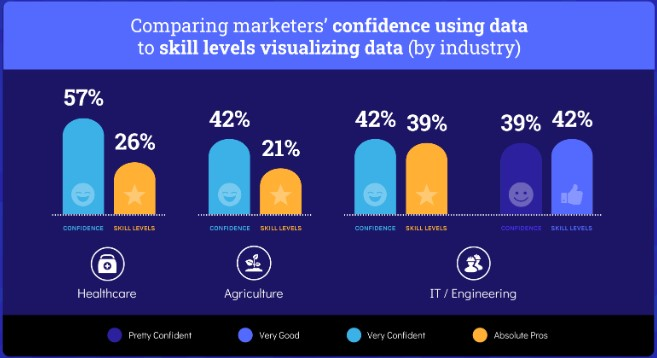
\includegraphics[width=6cm]{./images/3.jpg} 

 
 
\subsection{Data storytelling elements}
The so-called Data Storytelling is nothing more than a structured approach on how we communicate insights from data, and it involves a combination of three elements: data, visualization and narrative.\\
Now we can see the combination of these elements\\
\begin{center}
	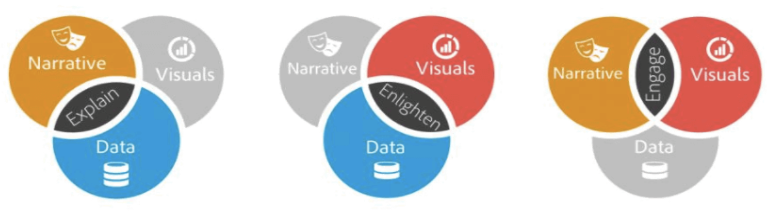
\includegraphics[width=8cm]{./images/1.png} 
\end{center}
\begin{itemize}
\item \textbf{Narrative + Data}
We will be able to explain what happened and why an insight may be important. We will need context to fully understand the conclusions.
\item \textbf{Visualization + Data}
When we add a visualization to our data, we can enlighten our audience with insights they might not have seen otherwise.
\item \textbf{Narrative + Visualization}
The perfect combination to achieve that interest and even to entertain our audience.
\item \textbf{Visualization + Narration + Data}
We managed to tell a story with our data, we managed to influence and lead to that change we were looking for.
\end{itemize}
\begin{center}
	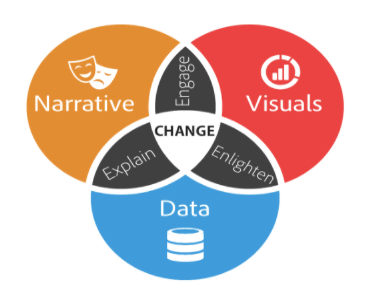
\includegraphics[width=8cm]{./images/2.png} 
\end{center}


\subsection{Business Examples}
Data Storytelling is not a new concept. Companies have been trying it for many years and have seen success. Here are some examples:
\subsubsection{Spotify}
\begin{center}
	
\includegraphics[width=7cm]{./images/5.jpg} 
\end{center}
Spotify, a music app, has sent annual summaries to its customers in email format. These short stories extract interesting statistics for each user, such as the number of minutes they have listened to music on their app.

\subsubsection{We Feel Fine by Jonathan Harris}
\begin{center}
	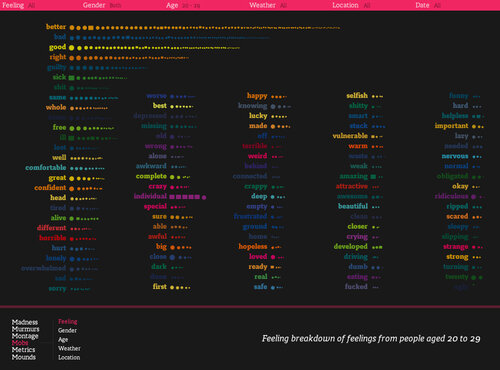
\includegraphics[width=7cm]{./images/4.jpeg} 
\end{center}
“An interactive website…that searches the internet every 10 minutes for expressions of human emotion on blogs and then displays the results in several visually-rich dynamic representations.

\subsubsection{Google Maps}
\begin{center}
	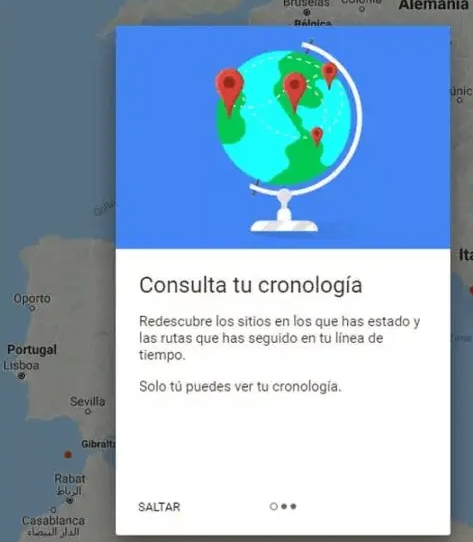
\includegraphics[width=7cm]{./images/6.png} 
\end{center}
Google Maps provides a monthly trip report to users who turn on the "Location History" feature on their mobile devices. It is possible to explore this feature by interacting with Google Maps.

You can know the places and cities that you visited the most, see photos taken in each location and acquire information about the most used means of transport.
 
 \subsubsection{Hospital John's Hopkins}
\begin{center}
	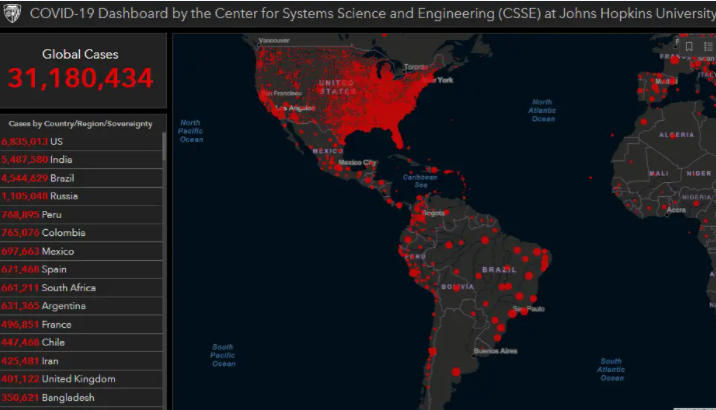
\includegraphics[width=7cm]{./images/7.png} 
\end{center}
When we are faced with a global pandemic, people all over the world receive a great deal of information on the subject on a daily basis.\\
Once again, fake news is a danger, so how can we be sure to collect all the necessary information from a reliable source?
\\
Johns Hopkins University Hospital of Maryland has created a real-time map showing relevant figures on the COVID-19 situation around the world.









\section{Conclusions}
\begin{itemize}
    \item Data Storytelling is a strategic tool that allows the information contained in the data to be communicated in a simpler way until the audience is persuaded. For its development, it considers three main elements: data, visualization and narrative, whose efficient combination allows us to understand the hidden message of the data.
    
    \item Data Storytelling is a structured approach to how we communicate insights from data. For organizations it is very important to include stories in the analysis, because it helps to easily understand and persuade to generate a change in people's actions.
    
    \item If there were many automated forms of data communication, they could not replace the essential elements of data storytelling done by data storytellers. In the future, there may be an influx of artificial intelligence and machine learning that will try to fill these gaps, but it is too early to say what role they will play in data storytelling in order to help decision-making in the digital organizations of the future.
    
\end{itemize}
 

\section{Recommendations}
\begin{itemize}
    \item It is recommended to use clear and concise language since the idea of investing in data-driven storytelling is to simplify the reading of huge and complex amounts of data.
    
    \item It is recommended to know the audience well. Knowing who we are targeting, what are the targets with whom we want to connect is essential. To this objective audience we should add another, which is the one to whom we present our proposal and, therefore, the one that makes decisions. Thus, for example, it is not the same that we do it before the senior executives of a company than before the head of marketing.
    
\end{itemize}
\end{multicols}
\newpage


\begin{thebibliography}{}

    \bibitem{DOC2008} 
    Matti, B. (2021, 21 de Septiembre) An Introduction to Data Storytelling - https://medium.com/big-data-today/an-introduction-to-data-storytelling-7a9bd986c7e9
    
    \bibitem{FRE2016} 
    Laura, B. (2020, 21 de Septiembre) Guía del Data Storytelling: cómo cautivar a tu audiencia con historias basadas en datos valiosos - https://rockcontent.com/es/blog/data-storytelling/
   
    \bibitem{FRE2019} 
    Zach, G. (2022, 17 de Febrero) 20 Best Data Storytelling Examples (Updated for 2022) - https://www.juiceanalytics.com/writing/20-best-data-storytelling-examples
  
    \bibitem{FRE2019}
    Empresa Actual (2021, 31 de Marzo) ¿Qué es el Data Storytelling? - https://www.empresaactual.com/que-es-el-data-storytelling/#:~:text=Data%20Storytelling%20dar%20un%20enfoque,%3A%20datos%2C%20visualizaci%C3%B3n%20y%20narrativa
    
    \bibitem{FRE2018}
    Venngage (2021, 18 de Febrero) How to Tell a Story With Data: A Guide for Beginners - https://venngage.com/blog/data-storytelling/
   
   \bibitem{FRE2018}
   Cyberclick (2021, 18 de Febrero) Data storytelling: ¿qué es y cómo contar buenas historias con datos? - https://www.cyberclick.es/numerical-blog/data-storytelling-que-es-y-como-contar-buenas-historias-con-datos
   
   \bibitem{FRE2018}
   Leila, S. (2019) Aprende a transformar datos en historias impactantes gracias al Data Storytelling - https://www.thepowermba.com/es/blog/data-storytelling
    
    \bibitem{FRE2018}
    KaitsConsulting (2018) Data storytelling: El valor del contexto y la narrativa para activar tus datos - https://www.kaitsconsulting.com/contexto-y-narrativa-para-activar-tus-datos/

    \bibitem{FRE2018}
    Merkile (2018) Data storytelling: Data Storytelling: qué necesitas saber - https://www.merkleinc.com/es/es/blog/data-storytelling#:~:text=Elementos%20clave,%3A%20datos%2C%20visualizaci%C3%B3n%20y%20narrativa

    \bibitem{FRE2018}
    Nogit (2018) What is Data Storytelling? - https://www.nugit.co/what-is-data-storytelling/
    

 
    \end{thebibliography
    
    


\end{document}


